\chapter{Experiments}
As we have covered, the effect of a Multi-Task problem setting is challenging to quantify theoretically without experiments.
Here we will take various datasets for object recognition, object detection, and pose estimation and see what the effects of training them in a Multi-Task setting are.
The metrics we are mainly interested in are the reduction in model size, inference time, and model accuracy on the different tasks compared to the single-task counterparts.
We will also attempt to find out how much more difficult the training process and tuning various hyperparameters are when compared to the single-task problem.
The experiments will focus on utilizing the previously presented EfficientNet and ResNet in various multi-task experiments to see how they compare.
The actual models will be EfficientNet-B3 and ResNet-101 since they require a roughly equivalent amount of memory to train.

\section{Training setup}
All the experiments use the same computer, and the model training is done using an Nvidia GeForce RTX 2070 GPU that has 8 GB of GDDR6 VRAM \citep{nvidiaRTX}.
Thus all the models will have to be small enough to train on this relatively small amount of memory.
The deep learning framework that is used to implement the models in all the experiments will be PyTorch \citep{pytorch} that is used inside Docker \citep{docker} containers.
Also, Nvidia Apex \citep{Apex} will be used to train models using mixed precision floating-point numbers to reduce the size of the models and to increase the speed of floating-point operations.
The model weights will be 16-bit floating-point numbers where it is safe to use the lower precision representation.
Besides the performance improvement, using lower precision floating-points can act as a regularizer as the model can't overfit on the high precision values and thus improve model accuracy as well \citep{mixedTraining}.

As a default for each task, we will use the following default procedures unless otherwise stated.
For the Multi-task training process, we will sample the data sets for each task with a probability respective to its size.
The loss function for every task has the same weight multiplier of one.
The batch size for each task will be maximized to fit within the memory requirement, giving a batch size of 32.
For weight optimizer, we will use SGD with a cyclic learning rate scheduler \citep{cycliclr}.

\section{Mixed precision training}

\section{Basic multiple object classification tasks}
As we have previously covered, fine-tuning an ImageNet classifier often produces good results.
Here we will take a pre-trained ImageNet backbone and learn multiple object classification tasks using the shared image embedding.
First, we will use two datasets that both contain images of healthy and unhealthy plants.

\begin{figure}[h!]
    \centering
    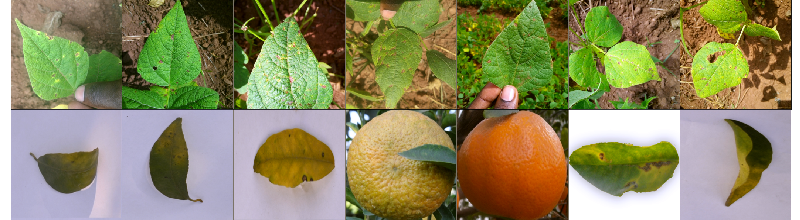
\includegraphics[width=0.8\textwidth]{imgs/citrus_beans_examples.png}
    \caption{Example images from the citrus and ibean data sets.
        The images in the top row are from ibean, and the bottom row is from the citrus data set.}
\end{figure}

The ibean dataset \citep{beansdata} contains 1296 images classified into three classes; Healthy, Angular Leaf Spot, and Bean Rust.
The data set provides a split for the images that will be the split that is used for the experiments.
The citrus leaves dataset \citep{citrusdata}, on the other hand, contains 759 examples of citrus fruits and leaves with six different classes; Black Spot, Canker, Greening, Scab, Melanose, and Healthy.
This set is quite tricky as it contains 609 images of leaves and only 150 images of actual citrus fruits, and some of the classes have very few images.
Some examples from the data sets are in Figure 7.1.
For the training split, the data will be split in 65/10/25 ratio for the training, validation, and test sets, respectively.
Both of these datasets have a relatively small amount of images available for training, so it should serve as a good basis for trying to train multi-task classifiers and give a glimpse into the adjustments that need to be made when training multi-task classifiers.
The goal for this experiment is to get familiar with the basics of how to create the multi-task models, and how to do the actual changes to the training loop in the Pytorch code to accommodate for the multi-task training.

When the two closely related datasets are used to train the model, we could expect the model to generalize better on both of them, as hopefully similar features would benefit both tasks.
But as the tasks are quite simple, the benefits can be relatively small as the likely accuracy for the single-task models should be quite high.
In the case of the citrus data set, learning to classify the citrus fruits could prove quite difficult, and for that, the bean leaves likely won't be of much help.
This model is depicted in figure 7.2.

\begin{figure}[h!]
    \centering
    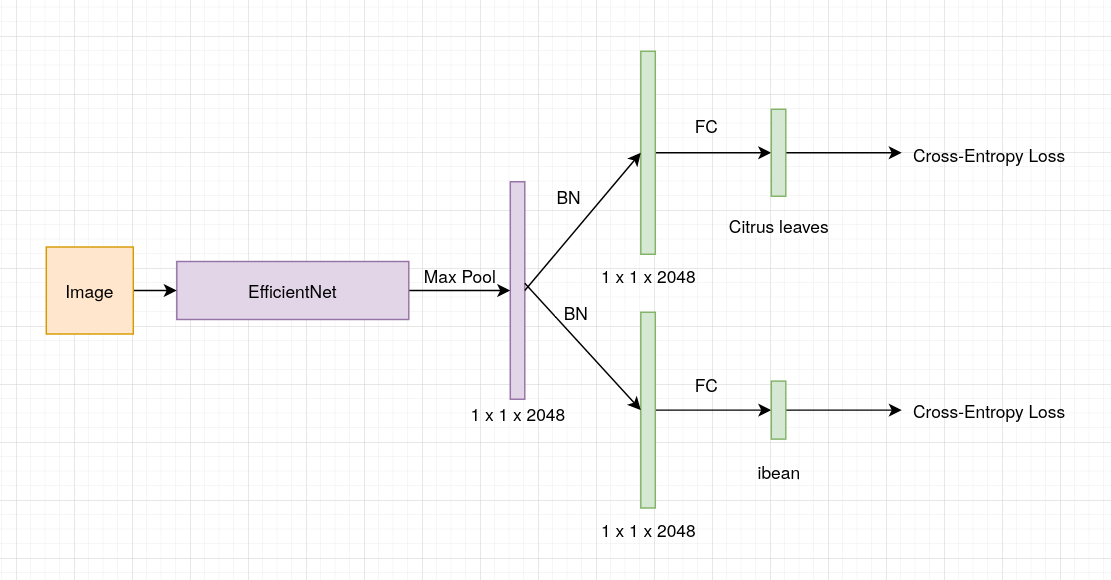
\includegraphics[width=0.8\textwidth]{imgs/object_classification_architecture.png}
    \caption{Network architecture for two image classification tasks.}
\end{figure}

To further extend the generalizability, we will try to add a third somewhat similar classification task using the Oxford flowers dataset \citep{flowers102}, which contains five different types of flowers.
The assumption here would be that flowers could require similar features as the previous leaf classification tasks, thus when increasing the training data with a closely related task, we could increase the generalizability even further.

Multi-task and single-task models were created and evaluated for both EfficientNet and ResNet backbones.
For the single-task performance, in this case, the ResNet model did slightly better on both of the tasks achieving 96\% test accuracy on the beans dataset and 88\% test accuracy on the citrus dataset, and the EfficientNet model achieved 94\% and 84\% test accuracies on the tasks.
In terms of training, the most significant parameter is the sampling ratio of the two tasks.

The sampling was done with a random number to pick which data loader would be used for the current batch.
If the sampling is done by going through each of the datasets entirely one at a time, the model ends up at a point where only one of the tasks has good accuracy.
If the ratio is left as proportional to the data set size, the multi-task model ends up only learning to classify the ibean data set, and the accuracy for the citrus data will stay low.
After some experimentation, the suitable probabilities for achieving good results with the EfficientNet multi-task classifier were 0.66 for the citrus and 0.33 for the ibean data.
Interestingly, the same ratio does not directly transfer to the ResNet model.
When using the same ratio as with the EfficientNet, the model still seems to converge only on a good result for the ibean data set.
For the final results with the ResNet classifier, the probability for the citrus dataset needed to be raised to 0.73.

\begin{table}[]
    \centering
    \begin{tabular}{lccl}
        \multicolumn{1}{l}{\textbf{}}    & \multicolumn{1}{l}{\textbf{ibeans}} & \multicolumn{1}{l}{\textbf{citrus}} & \multicolumn{1}{l}{\textbf{flowers}} \\ \cline{2-4}
        \textbf{Single-task models}      & \multicolumn{1}{l}{}                & \multicolumn{1}{l}{}                & \multicolumn{1}{c}{-}                \\ \hline
        \multicolumn{1}{l}{EfficientNet} & \multicolumn{1}{c}{94\%}            & \multicolumn{1}{c}{-}               & \multicolumn{1}{c}{-}                \\ \hline
        \multicolumn{1}{l}{EfficientNet} & \multicolumn{1}{c}{-}               & \multicolumn{1}{c}{84\%}            & \multicolumn{1}{c}{-}                \\ \hline
        \multicolumn{1}{l}{EfficientNet} & \multicolumn{1}{c}{-}               & \multicolumn{1}{c}{-}               & \multicolumn{1}{c}{97\%}             \\ \hline
        \multicolumn{1}{l}{ResNet}       & \multicolumn{1}{c}{96\%}            & \multicolumn{1}{c}{-}               & \multicolumn{1}{c}{-}                \\ \hline
        \multicolumn{1}{l}{ResNet}       & \multicolumn{1}{c}{-}               & \multicolumn{1}{c}{86\%}            & \multicolumn{1}{c}{-}                \\ \hline
        \multicolumn{1}{l}{ResNet}       & \multicolumn{1}{c}{-}               & \multicolumn{1}{c}{-}               & \multicolumn{1}{c}{97\%}             \\ \hline
        \textbf{Multi-task models}       & \multicolumn{1}{l}{}                & \multicolumn{1}{l}{}                & \multicolumn{1}{c}{-}                \\ \hline
        \multicolumn{1}{l}{EfficientNet} & \multicolumn{1}{c}{94\%}            & \multicolumn{1}{c}{88\%}            & \multicolumn{1}{c}{-}                \\ \hline
        \multicolumn{1}{l}{ResNet}       & \multicolumn{1}{c}{96\%}            & \multicolumn{1}{c}{89\%}            & \multicolumn{1}{c}{-}                \\ \hline
        \multicolumn{1}{l}{ResNet}       & \multicolumn{1}{c}{96\%}            & \multicolumn{1}{c}{91\%}            & \multicolumn{1}{c}{97\%}             \\ \hline
        \multicolumn{1}{l}{ResNet}       & \multicolumn{1}{c}{96\%}            & \multicolumn{1}{c}{-}               & \multicolumn{1}{c}{97\%}             \\ \hline
        \multicolumn{1}{l}{ResNet}       & \multicolumn{1}{c}{-}               & \multicolumn{1}{c}{85\%}            & \multicolumn{1}{c}{95\%}             \\ \hline
    \end{tabular}
    \caption{Accuracies on the data sets for both single-task and multi-task models with ResNet and EfficientNet.}
\end{table}

Training both tasks in a multi-task setting, we found that the accuracy on the citrus data set was increased, and ibean accuracy stayed the same.
Specifically, the accuracy for the EfficientNet classifier went up to 88\% and for ResNet up to 89\%.
The final model evaluated on the test set was the model with the highest average validation accuracy over the two tasks when trained for 25 epochs.
All the results are displayed in table 7.1.
The results show that even though these tasks were relatively simple and the accuracies for the single-task models were high, there was a benefit to be gained from multi-task training.
Here we mainly focused on getting good results on a fully shared backbone, and more experiments could be done by having fewer parameters shared between the tasks.
As an introduction to multi-task learning, the experiments show that picking the correct sampling ratio is extremely important for achieving desired results.
In that way, the sampling ratio seems quite unlike learning rate in that picking too small learning rate may lead to slow convergence but will most likely produce results in the end.
With the sampling ratio, it seems that the correct value needs to be found by experimentation, as a too low ratio for the citrus data gives accuracies that can be as low as 60\%.

Based on the results from the multi-task results on two tasks, I tried to add the third flower recognition task.
The flower recognition task has about 10 000 images and 102 classes, whereas the other two tasks have significantly less data and fewer classes.
On the two task experiment, it seemed that the sampling ratio should be relative to the task difficulty.
Here it would seem that the 102 class flower recognition should be much more difficult than the other two tasks, and I tried using sampling ratios in the range of about 0.5 to 0.7 for the flower task.
The best result achieved with these ratios was multiple percentage points below the single-task performance on all tasks.
However, when the flower task ratio was 0.1, it was possible to surpass the single-task results on all the tasks.
This training approach took significantly longer to converge to results.
The original sampling ratios converged in about five epochs to the best model, and the low flower ratio took about 50 epochs.
I started the training using the sampling ratio of 0.1 and decided to increase it up to 0.2 by the end of the training process.

When the training the model using the lower flower sampling ratio, it quickly converges close to the single-task performance on the two smaller tasks and slowly learns the flower task.
It is hard to say exactly why such low sampling ratios seemed to work.
Perhaps it has something to do with the difficulty of overfitting on a single task in a multi-task setting even though the small training set is seen so many times.
So the features for the smaller data sets are not just memorizing the pixels of the training set, but rather the features that generalize well.
Since the model already has good features for the smaller tasks and it is forced to find only a relatively minor shift in the parameters to learn the flower classification.
And seeing as the other tasks are improved as well, it shows that some of the features of the flower data are useful in the easier tasks.

From the three task models, the final model was picked as the one having the best average validation accuracy on all the tasks.
The final model wasn't just this model directly, though.
To get the final model, I froze all the shared weights and then did fine-tuning similar to what one might do when training a transfer learning classifier.
Having the model train on all the tasks using the frozen representations seemed to be useful.
The fine-tuning may be a good idea since, while training, the shared features are constantly shifting, and when one task is trained, it shifts the weights according to its gradients.
The other tasks won't have adjusted to the new, slightly shifted shared weights, which can lead to incorrect classifications.
When the shared weights are frozen, each of the task heads gets to learn the exact mapping from the shared representation to the outputs without them shifting during training.

All in all, these experiments validated the assumptions made about the multi-task training quite well.
Still, finding the sampling ratio is very laborious and not very intuitive.
This is why the results for the citrus and flower pair is a bit lower, since I spent less time finding the optimal ratios and mainly verified that it works as expected.
Perhaps it could be automated to get somewhat decent indications of what should be tried.
The problem, in the end, is that even if some kind of grid search could be applied, it would take very long to predict the final metrics of the models, and as seen in the discrepancy of the flower ratios, it could take many epochs to get the final results.
Perhaps some kind of dynamic sampling ratio, where the task lowest relative to the expected accuracy is sampled more, could be beneficial.

\section{Different tasks using shared representation}
Here we will create similar models to \citep{visualPerson}, but using EfficientNet, and then we will add a shared object detector to detect the people.

\section{Multiple object detectors}
Train multiple object detector using shared representations